\chapter{Umsetzung des neuronalen Netzes zur Erkennung von Interaktionen}
Im Rahmen des Praxisprojekts entstand ein Prototyp, welcher ein Sofa darstellt, das als Verwaltung von Interaktionen und Steuerung für smarte Endgeräte dient. Die Verwaltung erfolgt durch ein Regelsystem, welches durch ein ersetzt neuronales Netz werden soll. Der vierte Teil erläutert die Umsetzung von der Aufgabe eines neuronalen Netzes im Smart Home bis zu den Funktionen des neuronalen Netz zur Verwaltung der Interaktionen.

\section{Anforderungen an die Umsetzung}
Zu Beginn ist sehr wichtig zu erwähnen, dass die Echtheit der Werte aus der Außenwelt für ein neuronales Netz garantiert sein müssen. Kapitel \ref{subsec:ergeb} zeigt den Grund für diese Aussage. Dies wurde zu Beginn der Bachelorarbeit noch nicht bedacht, weshalb in Kapitel \ref{sec:ums_nn} auch noch andere Werte zur Verarbeitung verwendet werden. Daher ist es wichtig, dass diese Anforderung bei der Entwicklung erfüllt wird. Um Supervised Learning einzusetzen, muss das neuronale Netz einen Datensatz mit den Sensorwerten und einen weiteren Datensatz mit den entsprechenden Positionen einlesen. Weiterhin ist es wichtig, dass die Ergebnisse den Soll-Werten vollständig entsprechen, was mit dem neuronalen Netz in Kapitel \ref{ssec:nn_keras} aber noch nicht komplett der Fall ist. Um dies umsetzen zu können, braucht das neuronale Netz mehr Zeit für die Entwicklung und Verbesserung der Vorhersagen. Damit der Autor die Ergebnisse auswerten kann, ist es wichtig im Programm die Verbesserungen visualisiert werden, bei der Ausführung des Programms. Außerdem muss die Fehlerrate als Wert vorhanden sein, damit Differenzen bei unterschiedlichen Datensätzen zu sehen sind. Zuletzt ist es wichtig, dass das neuronale Netz am Ende so entwickelt ist, dass die Daten aus der Architektur aus Kapitel \ref{sec:arch_sofa} eingelesen werden können. \citep{frochte2018} bietet ein schon fertiges neuronales Netz, welches den Anforderungen zur erfolgreichen Ausführung des Netzes bietet. Das Netz muss entsprechend an den Datensatz angepasst werden, damit es die richtigen Ergebnisse liefert.

\section{Umsetzung des neuronalen Netzes mit Numpy}
\label{sec:ums_nn}
Das folgende Kapitel beschreibt die Umsetzung des neuronalen Netzes ohne eine Machine Learning Bibliothek. Die Vorgehensweise eine Python-Bibliothek für Machine Learning zu nutzen, kam erst als spätere Erkenntnis nachdem die Sensordaten über die empirische Methode gesammelt wurden. Da der Datensatz sehr groß ist und die Nutzung einer schon vorhanden Bibliothek ein Vorteil ist, um einfache Änderungen zur besseren Vorhersage vornehmen zu können, entsteht das neuronale Netz mit Keras erst ab diesem Zeitpunkt.
Der Aufbau eines solchen neuronalen Netzes und einer Erläuterung der einzelnen Funktionen und Komponenten, befinden sich in den Grundlagen in Kapitel \ref{sec:NNK} bei den Grundlagen. Mit dem entsprechenden Programmcode erläutert der Autor hier nur die Umsetzung des neuronalen Netzes mit Numpy.
\newline
\newline
Zu Beginn dieser Umsetzung wurde eine Funktion geschrieben, welche die sigmoid-Funktion beinhaltet. Diese wird in einer Trainingsfunktion aufgerufen. Die Trainingsfunktion ist der Hauptteil dieses neuronalen Netzes. 
\newline
Die nachfolgende Erklärung des Python-Codes beschreibt die Vorhersage mit drei Units im Input- und Output-Layer. Das komplette selbstgeschriebene neuronale Netz hat insgesamt drei Inputwerte und drei Outputwerte. 
\begin{python}
def train():
    with open("values.txt") as f:
        dataset = [[int(x) for x in line.split(",")] 
                    for line in f]
        print(dataset)
\end{python}
Als erstes gilt in dieser Funktion das Einlesen und Aufteilen der Textdatei. Danach folgt das Zusammenrechnen der Inputwerte mit den Gewichtungen und die daraus errechnete Summe für jede Unit. An dieser Stelle bekommt das neuronale Netz jeweils einen Inputwert pro Unit im Inputlayer. Zusätzlich wird an dieser Stelle noch der Bias-Wert dazu gerechnet.
\begin{python}
x = point[0] * w1 + point[1] * w2 + point[2] * w3 + b1
\end{python}
Ist die Summe ausgerechnet, werden die Ergebnisse in die sigmoid-Funktion übergeben und die Aktivierungsfunktion wird ausgelöst.
\begin{python}
pred1 = sigmoid(x)
\end{python}
Anschließend rechnet die Fehlerfunktion aus den Ergebnissen und dem gewünschten Ergebnis den mittleren quadratischen Fehler aus. Die Variable \emph{target} beschreibt das gewünschte Ergebnis.
\begin{python}
cost1 = np.square(pred1 - target1)
\end{python}
Das Ergebnis dieser Fehlerfunktion zeigt die Fehlerrate für die Vorhersagen mit den unveränderten Gewichtungen an. Als nächstes wird die Fehlerfunktion und sigmoid-Funktion abgeleitet.
Das \emph{d} vor den Namen steht im Code für Derived also abgeleitet. 
\begin{python}
dcost_dpred1 = 2 * (pred1 - target1)
dpred_dz1 = sigmoid_p(x)
\end{python}
Diese beiden Funktionen müssen nun anschließend multipliziert werden. Die dadurch entstehenden Ergebnisse müssen durch multiplizieren mit dem gewünschten Ergebnis zusammengerechnet werden. 
Um nun die Gewichte anzupassen, subtrahiert man das Gewicht mit der Lernrate von 0,1 und multipliziert diese mit der zuvor errechneten \emph{cost} Variable.
\newline
\begin{python}
dcost_dz1 = dcost_dpred1 * dpred_dz1
dcost_dw1 = dcost_dz1 * dz_dw1
w1 = w1 - learning_rate * dcost_dw1
\end{python}
Als weitere Erläuterung des Codes wird noch hinzugefügt, dass dieser Vorgang insgesamt 1000 Mal in einer \emph{for-Schleife} durchgeführt wird.
\newline
Für sehr kleine und einfach gehaltene Inputwerte kann dieses neuronale Netz verwendet werden. Da für das System aber acht Inputwerte genommen werden, müssten dementsprechend auch acht Gewichte benutzt und die Layer angepasst werden. Daher wird im nächsten Kapitel das neuronale Netz vorgestellt, welches mit Keras ausgeführt wird. Durch die Nutzung von Keras und TensorFlow sind größere neuronale Netze wesentlich simpler umzusetzen wie es in Kapitel \ref{ssec:nn_keras} vorgestellt wird.
\newline
\begin{figure}[H]
	\centering
		%[natürliche Breite in Pixeln, natürliche Höhe in Pixeln, Abhängigkeit von der Textbreite]
		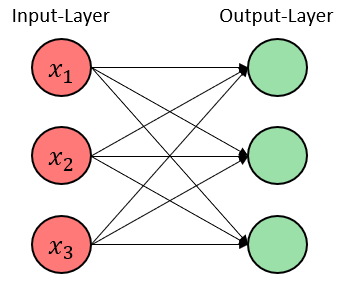
\includegraphics[width=0.4\textwidth]{images/einf_nn.png}
	\caption{Vereinfachtes neuronales Netz umgesetzt mit Numpy}
	\label{fig:einf_NN}
\end{figure}
\newline
Die Abbildung \ref{fig:einf_NN} zeigt die Architektur des neuronalen Netzes, welches mit Numpy umgesetzt ist. Die farblichen Markierungen zeigen die Units der Layer. Der Input-Layer ist rot und der Output-Layer ist grün. Wie schon erläutert werden hier nur drei Inputwerte eingegeben und vom Netz verarbeitet. Dies kann in der Architektur auch nochmal beobachtet werden.

\section{Umsetzung des neuronalen Netzes mit Keras}
\label{ssec:nn_keras}
In Kapitel \ref{sec:ums_nn} bildet sich die Erkenntnis, ein neuronales Netz mit Keras zu entwickeln, da die Art der Umsetzung mit Numpy eher für simplere Netze geeignet ist. Daher ist es wichtig, wie das neuronale Netz für den aktuellen Prototypen umgesetzt ist. 
\newline
\newline
Das neuronale Netz verwendet das Frontend Keras. Dies ist eine unterstützte Bibliothek von TensorFlow. TensorFlow ist das Backend und führt alle Berechnungen und Vorhersagen durch. Kapitel \ref{sec:tens} beschreibt dessen Aufbau und Funktion sowie die Verbindung zwischen Keras und TensorFlow. Da Keras eine Bibliothek für Python ist, ist das neuronale Netz auch entsprechend damit umgesetzt.
\newline
Als Ergänzung zu der Erklärung aus den Grundlagen \ref{sec:NNK} ist noch erweitert zu erläutern, dass das neuronale Netz zum Training in diesem Projekt Datensätze aus CSV-Dateien einliest. Die Testdaten werden aus den Datasets als zufällige Anzahl ausgewählt. Insgesamt gibt es pro Proband immer eine CSV-Datei für seine Interaktionen auf dem Sofa und eine zweite CSV-Datei für die entsprechenden Vorhersagen. Kapitel \ref{sec:dataset} beschreibt den Aufbau der CSV-Dateien. Da für das neuronale Netz Datensätze benutzt werden, welche vom Prototypen erstellt werden, normalisiert das neuronale Netz die Daten. An diesem Punkt hat Keras auch eine eigene Funktion, die dafür aufgerufen wird.
\newline
Das Fully-connected Neural Network ist untereinander mit allen vorherigen Schichten verbunden. Zu Beginn muss ein Sequential-Objekt in Python deklariert werden, damit das neuronale Netz Schicht für Schicht aufgebaut werden kann. Im nachfolgenden Code-Abschnitt werden die Layer des neuronalen Netzes deklariert. Die Funktionsaufrufe \emph{myANN.add(Dense())} sind die einzelnen Layer und mit der \emph{BatchNormalization()} werden die Ergebnisse aus dem vorherigen Layer normalisiert. In Keras wird dieser Aufruf zur Normalisierung wie ein Layer dargestellt. Die Aktivierungsfunktion des Hidden-Layers und Output-Layers ist die sigmoid-Funktion. Außerdem wird der optionale Parameter angegeben, dass die Bias-Unit benutzt werden soll. Der Hidden-Layer ist zu Beginn mit der Rectified Linear Units-Funktion entstanden. Mit dieser Funktion entstand eine Fehlerrate von 72\%, was mit der sigmoid-Funktion nicht der Fall ist. Diese Funktion gibt bei Ergebnissen kleiner Null den Wert Null aus und alle Werte darüber werden als dessen Werte ausgegeben. Die weiteren Ergebnisse sind in Kapitel \ref{subsec:ergeb} aufgeführt und werden dort diskutiert.
\begin{python}
myANN.add(Dense(8, input_dim=8, 
                kernel_initializer='normal'))
myANN.add(Dense(8, kernel_initializer='normal', 
                activation='sigmoid', use_bias=True))
myANN.add(BatchNormalization())
myANN.add(Dense(3, kernel_initializer='normal', 
                activation='sigmoid', use_bias=True))
\end{python}
Als Fehlerfunktion wird Mean Squared Error verwendet und Adam als Optimizer. Aus den Versuchen, die Fehlerrate so gering wie möglich zu halten, stellt sich für den Mean Squared Error und die Learning Rate vom Adam Optimizer ein Wert von 0,001 als beste Wahl heraus. Die Umsetzung des neuronalen Netzes stammt aus einer Vorlage aus dem Buch \citep{frochte2018} und wurde auf den Trainingsdatensatz vom Sofaprototypen angepasst. Das Python-Programm befindet sich in Kapitel \ref{cha:anh} als Anhang. Zuletzt wird im neuronalen Netz die \emph{matplotlib.pyplot} importiert. So werden die Veränderungen während des Trainings zur Fehlerfunktion in einem Koordinatensystem dargestellt.
\newline
\begin{figure}[H]
	\centering
		%[natürliche Breite in Pixeln, natürliche Höhe in Pixeln, Abhängigkeit von der Textbreite]
		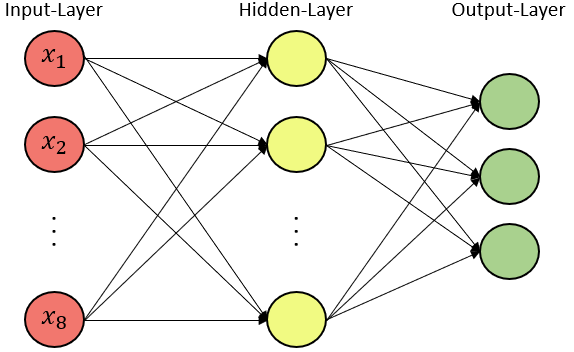
\includegraphics[width=0.6\textwidth]{images/NN.png}
	\caption{Darstellung des neuronalen Netzes zur Verwaltung der Interaktionen}
	\label{fig:NN}
\end{figure}
\newline
Abbildung \ref{fig:NN} zeigt die Architektur des neuronalen Netzes, welches mit Keras entwickelt wurde. Insgesamt hat der Input- und Hidden-Layer acht Units und der Output-Layer drei Units. Es werden insgesamt acht Inputwerte in Form von Sensordaten im Input-Layer eingegeben und verarbeitet. Die entsprechenden Layer sind zur besseren Unterscheidung farblich markiert. Die Units im Input-Layer sind rot, die Units im Hidden-Layer sind gelb und die Units Output-Layer sind grün. Die Bias-Unit wird hier nicht dargestellt, wird aber trotzdem im Hidden- und Output-Layer als zusätzlicher Wert dazu gerechnet. Wie Keras und TensorFlow funktionieren und in Beziehung zueinander stehen, hat der Autor dies im nächsten Kapitel erläutert.

\section{Die Backend-Engine TensorFlow}
\label{sec:tens}
TensorFlow ist ein Open-Source Projekt, welches sich auf Deep Neural Networks spezialisiert. Das neuronale Netz verwendet TensorFlow 2 und Keras 2.3.0. TensorFlow ist eins der möglichen Backend Bibliotheken neben Microsoft Cognitive Toolkit und Theano. \citep{goldsborough2016tour} erläutert den Aufbau von Tensorflow und beschreibt dessen Elemente. Da TensorFlow für sehr große neuronale Netze ausgelegt ist, nutzt der Autor mit Keras den Vorteil, dass man nicht direkt mit TensorFlow arbeitet. So wird die Backend Bibliothek sehr einfach gehalten und ist von dessen Möglichkeiten übersichtlicher. Um die Unterschiede zu zeigen, wie mit TensorFlow direkt gearbeitet wird, zeigt \citep{santanu2017} in Kapitel 2. Wie Keras genutzt wird, zeigt die Umsetzung im Anhang. Abbildung \ref{fig:stack} zeigt nochmal den Aufbau und die Beziehung zwischen Keras und TensorFlow. Um TensorFlow zu benutzen, muss CUDA/cuDNN auch zusätzlich installiert werden. 

\begin{figure}[H]
	\centering
		%[natürliche Breite in Pixeln, natürliche Höhe in Pixeln, Abhängigkeit von der Textbreite]
		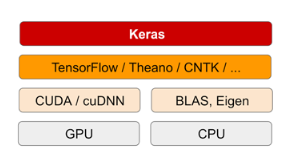
\includegraphics[width=0.6\textwidth]{images/dl_soft_hard.png}
	\caption{Der Software und Hardware Stack von Keras \citep{chollet2018}}
	\label{fig:stack}
\end{figure}

\section{Neue Funktionen durch das neuronale Netz}
\label{sec:new_func}
Die Hauptmerkmale zur Erkennung der Interaktionen verändern sich nicht vom Regelsystem aus gesehen mit dem neuronalen Netz. Das Regelsystem bestimmt anhand der Sensorwerte, welche Position der Nutzer auf dem Sofa einnimmt. Dies funktioniert nur, wenn die Personen immer für die von ihnen gewollte Steuerung die gleichen Sensoren besetzen.
\newline
Diese statische Steuerung wird durch das neuronale Netz zu einer dynamischen Verwaltung umgestaltet. Durch die Trainingsdaten wird im neuronalen Netz immer eingelesen wann eine Person sitzt, liegt oder das Sofa leer ist, egal wie sie auf dem Sofa diese Positionen ausführt. Das hat den Effekt, dass jede Person selber entscheiden kann, wie sie sich auf das Sofa setzen möchte. Dadurch kann trotzdem immer das gleiche smarte Gerät oder die entsprechende Automatisierung ausgelöst werden. Zudem muss bei neuen Liegepositionen und Sitzpositionen keine Regel aktualisiert oder hinzugefügt werden, da das neuronale Netz auch neue Interaktionen durch neue Nutzer erkennt. 
\newline
Für die Liegepositionen werden mit dem Regelsystem auch keine eigenen Sensoren verwendet, da die verschiedenen Liegepositionen vom neuronalen Netz erkannt werden und sie von Sitzpositionen unterscheiden. Ein weiterer Vorteil ist das Wegfallen des Flex-Sensors, da das neuronale Netz auch anhand der FSR-Sensoren erkennt, ob ein Nutzer liegt. Auf den Sitzkissen wird nur noch ein Sensor benötigt. Zudem ist es mit Flex-Sensoren sehr schwer zu erkennen, ob eine Person mit ihm interagiert, da dieser erst den Widerstand ab einer 45-Grad-Biegung messen kann. Durch das neuronale Netz fällt der Flex-Sensor weg und die Interaktionen können dynamisch verwaltet werden. Durch das Entfernen des Flex-Sensors wird der ESP8266 nicht mehr gebraucht, was die Erkennung der Sensordaten einheitlich gestalten lässt. Denn es wird nur noch der ESP32 benutzt. Wenn der Prototyp nur noch FSR-Sensoren besitzt, müssen unterschiedliche Sensorwerte nicht mehr verwaltet werden, was die Messung neuer Sensorwerte stark vereinfacht.

\section{Einbindung des neuronalen Netzes in den Prototypen}
\label{sec:einb}
Die Erkennung von Interaktionen findet über die Klassifizierung des neuronalen Netzes statt. Anhand der Ergebnisse aus dem Feedforward-Schritt und der darauf folgenden Backpropagation klassifiziert das neuronale Netz wie der Nutzer mit dem Sofa interagiert. Ist diese Aufgabe abgeschlossen und liefert die gewünschten Ergebnisse, besteht die Möglichkeit es in das Python-Programm einzubinden. Das Python-Programm ist im Anhang zu finden. Damit werden das Netz und das Python-Programm zur Erfassung der Sensorwerte auf dem Raspberry Pi zusammen mit dem MQTT-Broker ausgeführt. 
\newline
Wenn diese Klassifizierung mit den Testdaten immer richtig liegt, soll das neuronale Netz in das System des Sofaprototypen eingebunden werden. Durch die Zusammenführung entsteht jedoch der Punkt, dass ein Programm mehrere Aufgaben übernimmt. Deswegen will der Autor nicht unerwähnt lassen, dass es eher von Vorteil ist, wenn das neuronale Netz und das Python-Programm separat ausgeführt werden, damit jede Komponente nur eine Aufgabe hat.
\newline
Um zu prüfen, wie das Netz die Vorhersagen genauer treffen kann, beschreibt Kapitel \ref{sub:res} die Ergebnisse der Datensätze und welche für das Lernen am besten geeignet sind. Bevor diese Einbindung in den Prototypen stattfindet, muss das neuronale Netz erst noch weiter verbessert werden. Dies wird im folgenden Kapitel erläutert.

\section{Weiterführung der Entwicklung des neuronalen Netzes}
Aus Zeitgründen kann das neuronale Netz nicht so weiter entwickelt werden, dass dessen Vorhersagen immer stimmen. Dieses Kapitel soll in der Theorie beschreiben, was noch implementiert oder geändert werden muss, damit die Vorhersagen besser werden.
\newline
\newline
Neben der sigmoid- und ReLU-Funktion bietet TensorFlow viele weitere Aktivierungsfunktionen. Dabei muss immer beachtet werden, dass die Aktivierungsfunktion am Ende Werte ausgeben muss, welche Richtung null oder eins gehen. Dies muss aus dem Grund beachtet werden, weil im Ergebnisvektor pro Wert maximal eins oder null steht. Da die Lernrate vom größeren zum kleineren Wert gemessen wird, ist es möglich auch diese noch weiter anzupassen. Weiterhin gibt es mehrere Fehlerfunktionen, welche noch nicht getestet wurden, womit es aber auch möglich ist, das neuronale Netz weiter anzupassen.

\section{Verbesserungen des Prototypen}
\label{sec:verbesserungen}
In Kapitel \ref{cha:arch_pro} sind die Kernkomponenten des Prototypen aus dem Praxisprojekt erläutert. Zudem wird dort die Architektur des weiterentwickelten Prototypen visualisiert und erläutert. Kapitel \ref{sec:new_func} beschreibt daraufhin die mit dem neuronalen Netz einhergehenden Funktionen. Die daraus resultierenden Verbesserungen sind Möglichkeiten zur Verwaltung der Interaktionen. Außerdem werden Interaktionen besser erkannt und können auf verschiedene Arten die smarten Geräte steuern. Der Autor möchte hervorheben, dass das neuronale Netz für eine solche Steuerung die bessere Wahl ist als ein statisches Regelsystem, welches keine veränderten Interaktionen mit der Steuerung erlaubt. Zudem besteht die Möglichkeit die Interaktionen mit dem Sofa vielfältiger zu gestalten, um mehr Geräte und Abläufe zu Automatisieren. 
\newline
\newline
Die Kommunikation zwischen den Geräten bleibt auch bei der Nutzung eines neuronalen Netzes gleich. Die weitreichensten Unterschiede sind die Ergebnisse zur Steuerung der smarten Endgeräte und das Einbinden einer CSV-Datei, um das neuronale Netz trainieren und testen zu können. Hier wird das neuronale Netz auch nicht sofort in das Python-Programm eingebunden, so wie beim früheren Regelsystem. Es wird stattdessen als eigene Komponente ausgeführt und kommuniziert mit dem Python-Programm.
